\chapter{SYSTEM ANALYSIS AND DESIGN}

\section{Introduction}
\par
This chapter provides an explanation of our project design in the following sections: analysis of the existing system, diagram, system architecture, system design, and user interface design.

\section{Analysis of the existing system}
\par
The scope of this project is centered on King Mongkut’s University of Technology Thonburi (KMUTT) as the designated target area. The primary user groups are the personnel within the organization.

\section{User Requirement Analysis}
\subsection{User Requirements}
\par
The following are the functional specifications that users expect from the LostNFound KMUTT platform:
\begin{enumerate}
    \item \textbf{Lost and Found Item Reporting:} The system should allow users (students and university staff) to report lost and found items. Users should be able to submit detailed descriptions for the items they are reporting. This information is essential for accurate matching.
    \item \textbf{Item Matching:} The platform should use advanced text-matching techniques, such as Natural Language Processing (NLP), to compare lost and found item descriptions and ensure the correct matching between them. This allows users to easily identify and claim their belongings.
    \item \textbf{Secure Claim Process:} The system must verify users' identities using their \textbf{university email} to ensure only the rightful owner can claim an item. The platform should reject any claims from users who cannot prove ownership of the lost item.
    \item \textbf{History of Claimed Items:} The system needs to maintain a detailed record of all claimed items, including the name and ID of the user who claimed the item. This helps provide accountability and keeps a history of item claims for future reference.
    \item \textbf{Notification System:} Users should receive timely notifications when a match is found for their lost item or when they are reminded to pick up an item they have claimed.
    \item \textbf{Authentication and Security:} The system must ensure secure authentication using \textbf{Microsoft Extra ID} to authenticate users. Only users with valid \textbf{KMUTT email accounts} should be able to access the platform and participate in reporting or claiming items.
\end{enumerate}

\section{System design}
\subsection{Proposed Architecture Diagram}
\begin{figure}[!h]
    \centering
    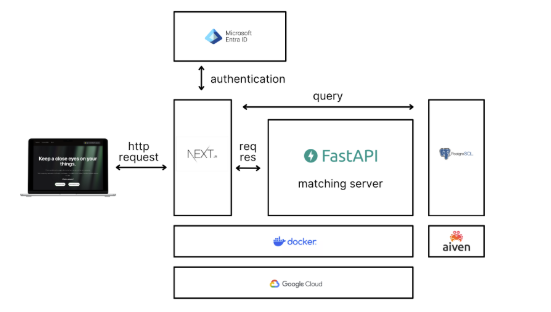
\includegraphics[width=1\linewidth]{chapter3/architecture-diagram.png}
    \caption{Architecture Diagram}
    \label{fig:Architecture Diagram}
\end{figure}
\par Figure 3.1 represents our system architecture. The platform will leverage Google Cloud Platform (GCP) for hosting, with Cloud Registry used for storing Docker images, and Cloud Build for automating the build process. The application will run on Cloud Run, providing a serverless environment for deploying containerized applications. For frontend development, we will use Next.js with Tailwind CSS for responsive and stylish web pages. The backend will be developed with FastAPI, which will expose NER and Text Similarity APIs for matching lost and found items. PostgreSQL will be used for storing data related to users and items, hosted on Aiven for managed database services. Docker will be utilized for containerizing the entire application, enabling efficient deployment and scalability within the cloud environment.

\newpage
\subsection{Context Diagram}
\begin{figure}[!h]
    \centering
    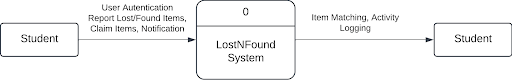
\includegraphics[width=1\linewidth]{chapter3/context-diagram.png}
    \caption{Context Diagram of LostNFound System}
    \label{fig:Context Diagram of LostNFound System}
\end{figure}
\par This figure shows the context diagram for the LostNFound KMUTT system. The diagram illustrates the overall interactions between the users and the system. Users (students and staff) are required to authenticate via their KMUTT email to access the platform. Once authenticated, students can report lost and found items. The core interactions of the system include the submission of item reports, matching items using \textbf{Text Similarity and NER APIs}, and the ability for users to track and claim their lost belongings.

\subsection{Data Flow Diagram}
\begin{figure}[!h]
    \centering
    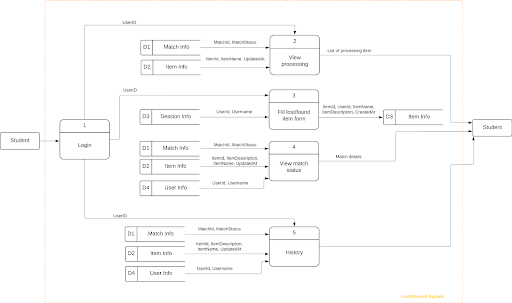
\includegraphics[width=1\linewidth]{chapter3/data-flow-diagram.png}
    \caption{Diagram 0}
    \label{fig:Diagram 0}
\end{figure}
\par
Figure 3.3 represents the data flow diagram of the LostNFound KMUTT system. The process starts when the user inputs their KMUTT email and password to authenticate. Once authenticated, the user can report a lost or found item by providing item details, such as description, location, and timestamp. The system processes and stores the data in the PostgreSQL database. Users can then view item matches using NLP for text similarity, claim found items, and receive notifications when a match is found or when they need to pick up their claimed item.

\newpage
\subsection{Activity Diagram}
\begin{figure}[!h]
    \centering
    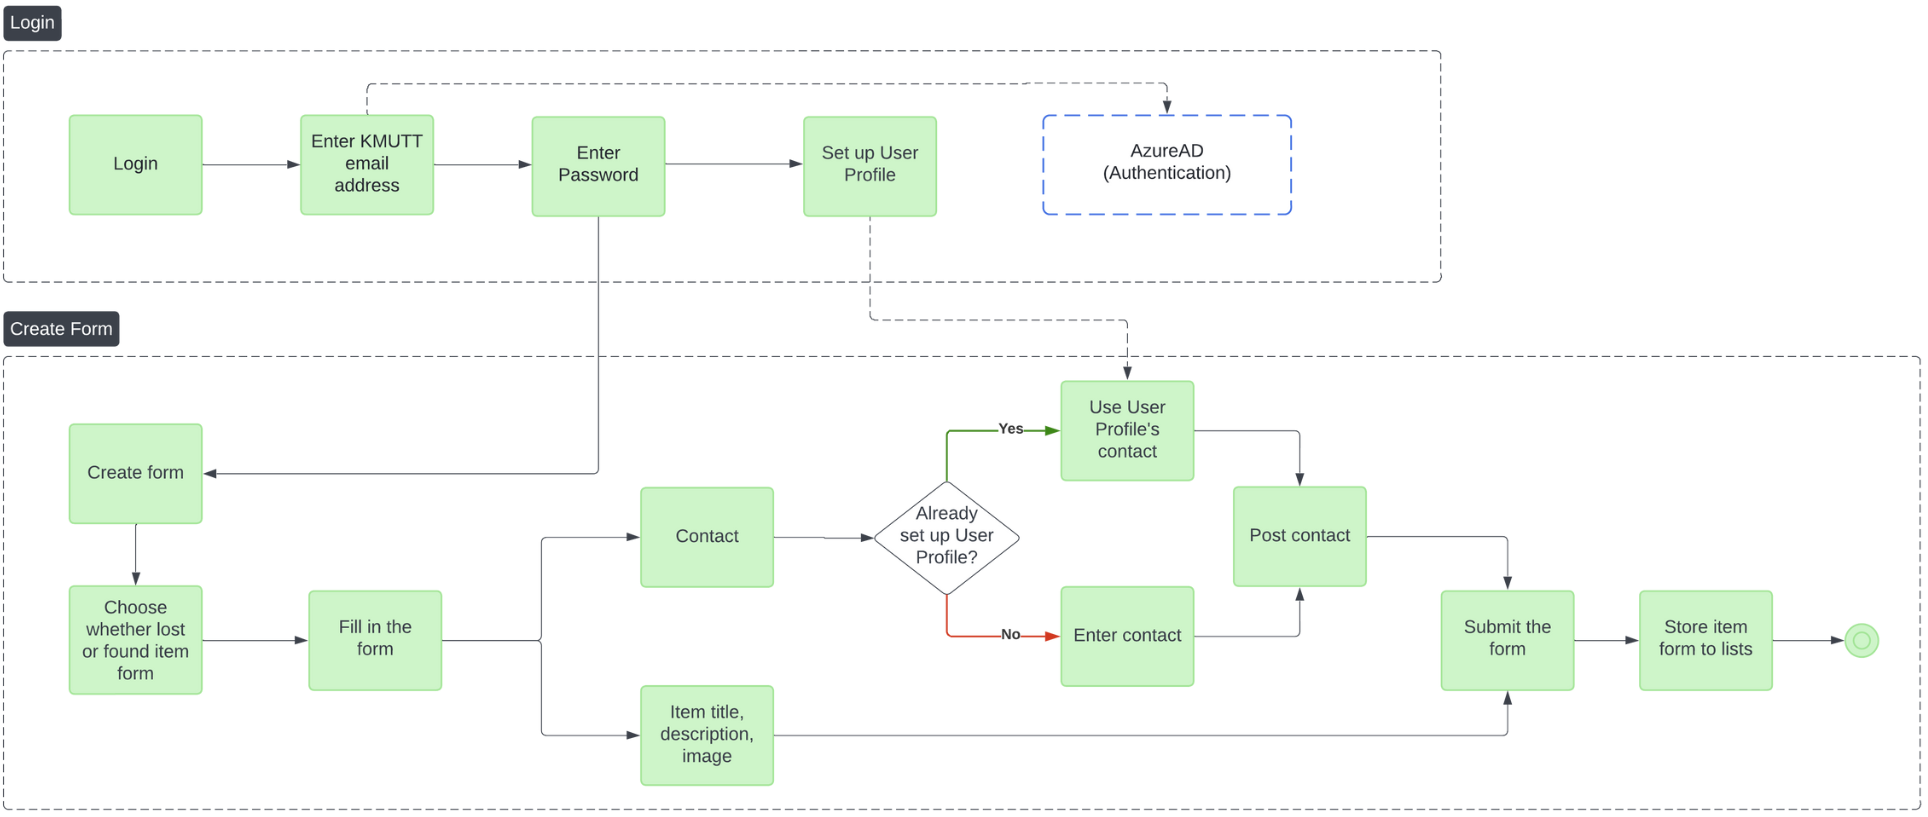
\includegraphics[width=1\linewidth]{chapter3/activity-diagram.png}
    \caption{Activity Diagram for student logins and creating lost or found item form of LostNFound System}
    \label{fig:Activity Diagram for student logins and creating lost or found item form of LostNFound System}
\end{figure}
\par
Figure 3-4 represents the flow when the student uses a web application by logging in with Microsoft Extra ID authentication. Once authenticated, the student is directed to the form page where they can choose to create a lost item or found item form. The student fills in the required details, including the item description. After submission, the form data is processed and stored in the system, where it can be used for matching with other lost or found items.

\newpage
\begin{figure}[!h]
    \centering
    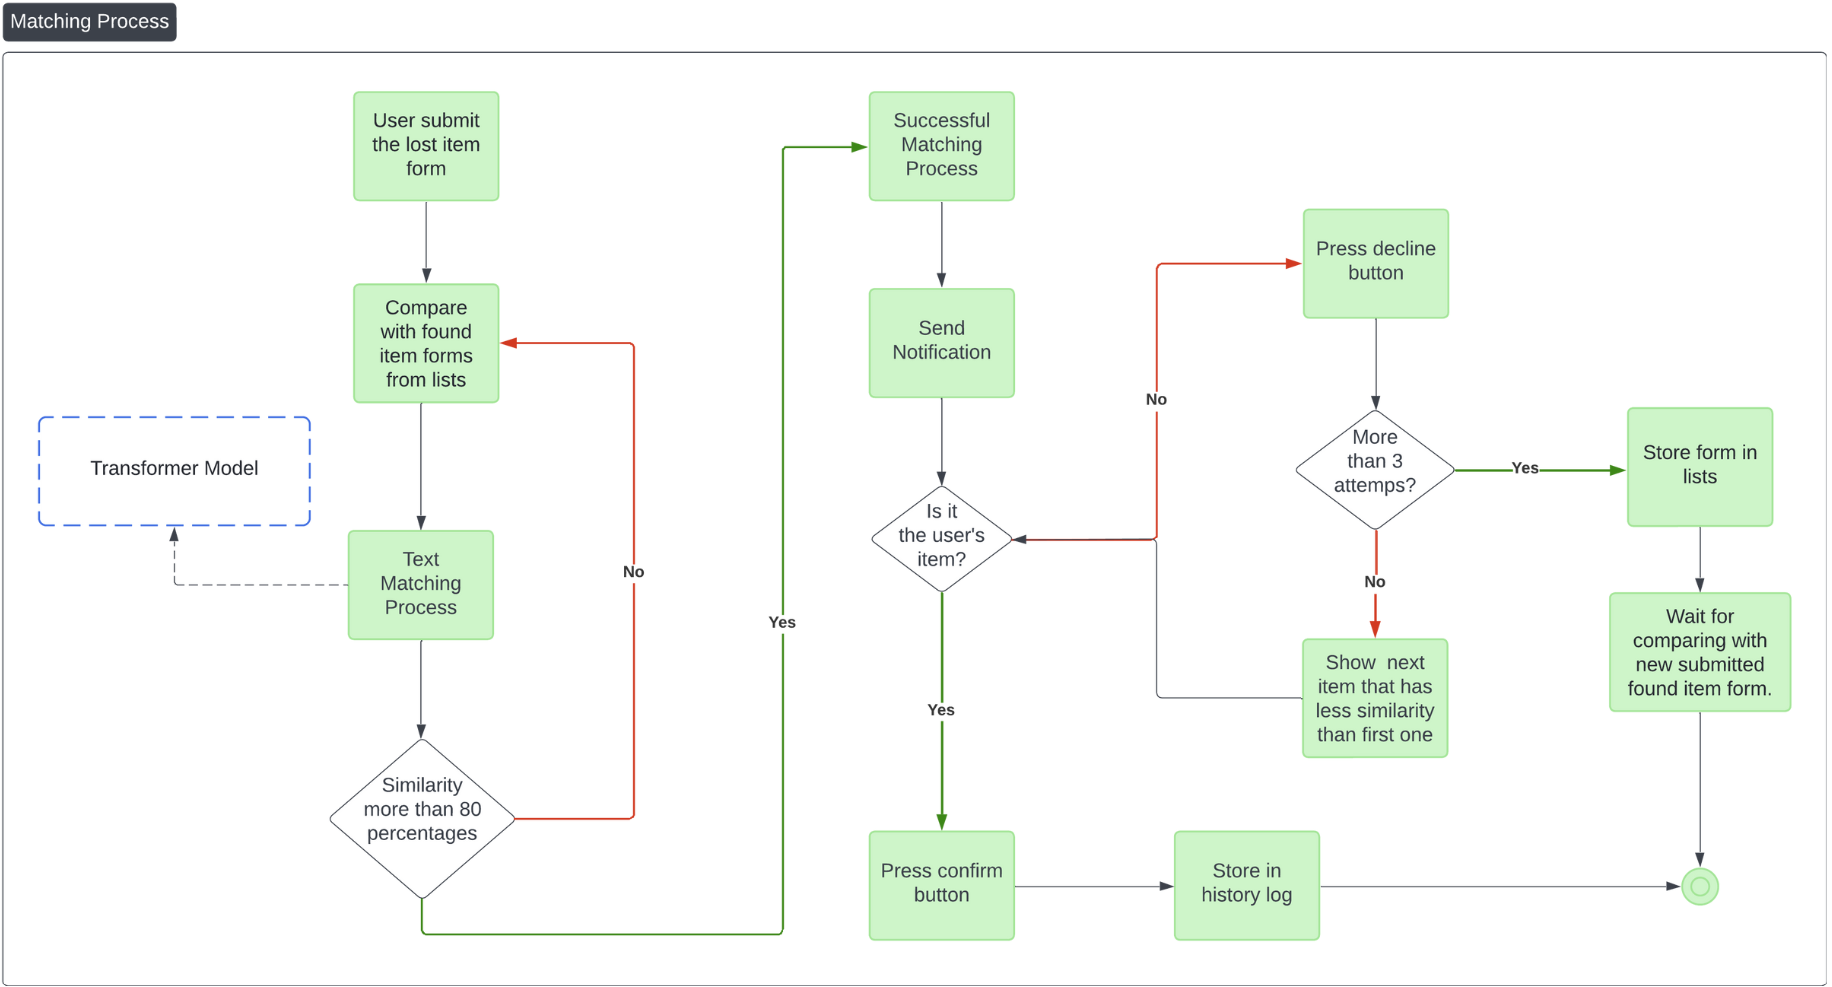
\includegraphics[width=1\linewidth]{chapter3/activity-diagram2.png}
    \caption{Activity Diagram for a matching process of LostNFound System}
    \label{fig:Activity Diagram for a matching process of LostNFound System}
\end{figure}
\par
Figure 3.5 represents the matching process in the LostNFound KMUTT system. The process begins when a lost item report or a found item report is submitted by a student or staff member. Once the report is submitted, the system uses Natural Language Processing (NLP) and Text Similarity algorithms to compare the item descriptions. The system processes key details such as description, product name, and location to identify potential matches.

\newpage
\begin{figure}
    \centering
    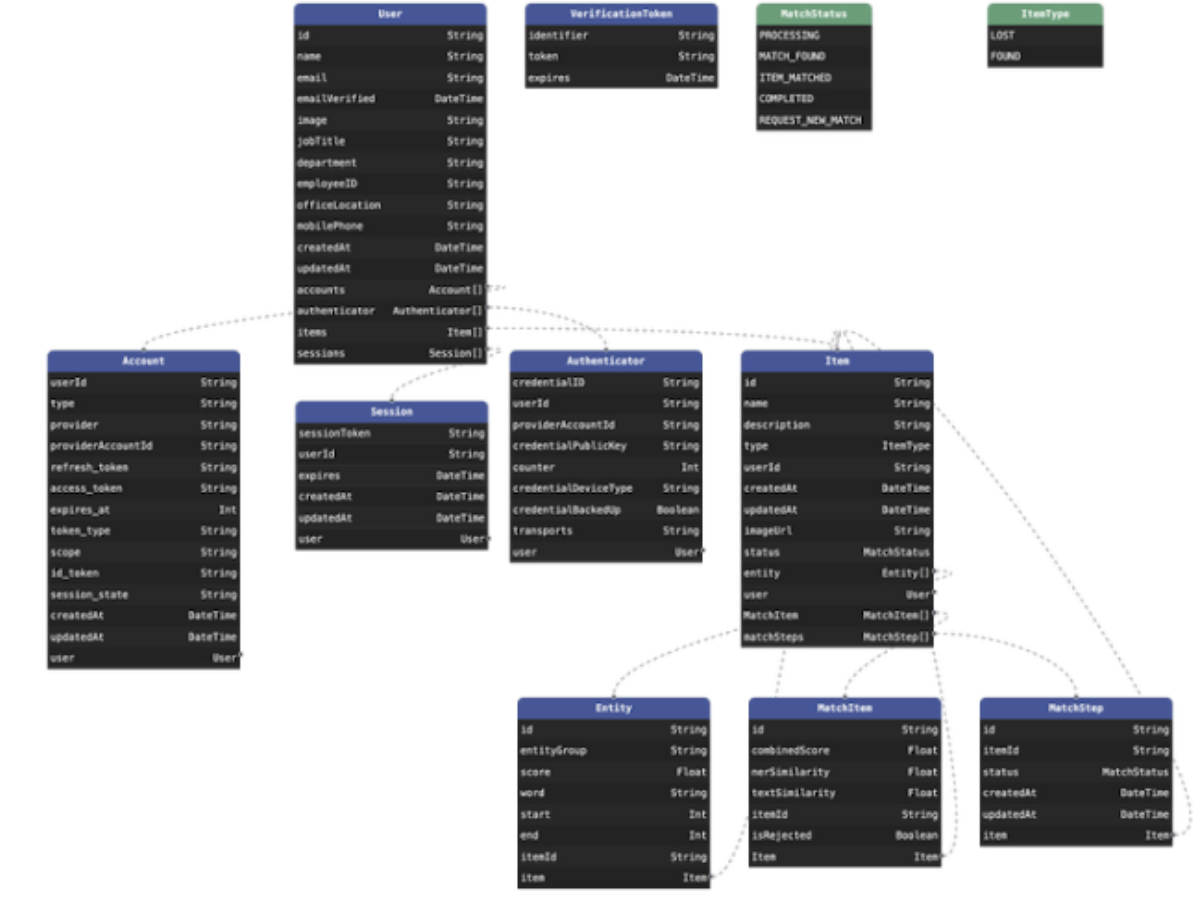
\includegraphics[width=1\linewidth]{chapter3/er-diagram.png}
    \caption{ER Diagram of LostNFound System}
    \label{fig:ER Diagram of LostNFound System}
\end{figure}
\par
Figure 3.6 represents the conceptual diagram of the LostNFound System which we will use to store information about users and match details.